\documentclass[10pt,openany]{book}
\usepackage[utf8]{inputenc}
\DeclareUnicodeCharacter{2212}{\ensuremath{-}}
\DeclareUnicodeCharacter{2192}{\ensuremath{\to}}
\DeclareUnicodeCharacter{03B1}{\ensuremath{\alpha}}
\usepackage[T1]{fontenc}
\usepackage{lmodern}
\AtBeginDocument{\normalfont\DeclareFontShape{T1}{lmr}{bx}{sc}{<->ssub*lmr/m/sc}{}}
\usepackage[spanish,es-nodecimaldot]{babel}
\spanishplainpercent
\AtBeginDocument{\spanishdeactivate{"~<>}}
\usepackage[a4paper,margin=2.5cm,headheight=14pt]{geometry}
\usepackage{amsmath,amssymb,mathtools,booktabs,array,longtable,graphicx,xcolor,tikz,enumitem,microtype,titlesec,fancyhdr}
\usepackage[breakable,skins]{tcolorbox}
\usepackage[labelfont=bf]{caption}
\usepackage[hyphens]{url}
\usepackage[hidelinks,unicode,hypertexnames=false]{hyperref}
\definecolor{studiumInk}{RGB}{20,44,64}
\definecolor{studiumBlue}{RGB}{24,74,130}
\definecolor{studiumCyan}{RGB}{0,184,205}
\definecolor{studiumLight}{RGB}{232,240,250}
\definecolor{studiumWorkedBack}{RGB}{255,244,230}
\definecolor{studiumWorkedFrame}{RGB}{138,78,12}
\definecolor{studiumCheckBack}{RGB}{243,236,248}
\definecolor{studiumCheckFrame}{RGB}{96,48,130}
\titleformat{\chapter}[display]{\normalfont\filright}{\large\mdseries\scshape\chaptertitlename\ \thechapter}{1ex}{\normalfont\huge\bfseries}
\titlespacing*{\chapter}{0pt}{2.5ex plus 1ex minus .2ex}{2.3ex}
\titleformat{name=\chapter,numberless}[display]{\normalfont\filright}{}{0pt}{\normalfont\huge\bfseries}
\titleformat{\section}{\Large\bfseries}{\thesection}{.8em}{}
\titleformat{\subsection}{\large\bfseries}{\thesubsection}{.7em}{}
\makeatletter
\renewcommand*\l@section{\@dottedtocline{1}{1.5em}{3.5em}}
\makeatother
\setcounter{secnumdepth}{2}\setcounter{tocdepth}{1}
\setlength{\parindent}{1.5em}\setlength{\parskip}{3pt plus .5pt}
\setlength{\emergencystretch}{1.5em}\raggedbottom
\setlist{itemsep=2pt,topsep=4pt,leftmargin=*}
\setlist[description]{style=nextline,leftmargin=0pt,labelwidth=0pt,labelindent=0pt}
\allowdisplaybreaks[2]
\graphicspath{{../figures/}}
\newcommand{\Raire}{287.05287}
\newcommand{\gzero}{9.80665}
\tcbset{studiumcommon/.style={breakable,boxrule=.65pt,arc=.7pt,left=1.7mm,right=1.7mm,top=1.3mm,bottom=1.3mm,before skip=10pt,after skip=10pt,fonttitle=\bfseries}}
\newtcolorbox{studiumworked}[1]{studiumcommon,colback=studiumWorkedBack,colframe=studiumWorkedFrame,colbacktitle=studiumWorkedFrame,coltitle=white,title={#1}}
\newcommand{\objetivos}[1]{\par\noindent\textbf{Objetivos de aprendizaje.} \textit{#1}\par\medskip}
\newcommand{\caja}[2]{\begin{tcolorbox}[studiumcommon,colback=studiumLight,colframe=studiumBlue,colbacktitle=studiumBlue,coltitle=white,title={#1}]#2\end{tcolorbox}}
\newcommand{\resumen}[1]{\begin{tcolorbox}[studiumcommon,colback=studiumCheckBack,colframe=studiumCheckFrame,colbacktitle=studiumCheckFrame,coltitle=white,title=Resumen]#1\end{tcolorbox}}
\newcommand{\figura}[2]{\begin{figure}[tbp]\centering\includegraphics[width=.83\linewidth]{#1.pdf}\caption{#2}\label{fig:#1}\end{figure}\noindent La figura~\ref{fig:#1} ofrece una representación del modelo discutido.}
\pagestyle{fancy}\fancyhf{}
\fancyhead[LE]{\small\thepage\hspace{1.5em}\mdseries\scshape\nouppercase{\leftmark}}
\fancyhead[RO]{\small\mdseries\scshape\nouppercase{\rightmark}\hspace{1.5em}\thepage}
\renewcommand{\headrulewidth}{.4pt}\renewcommand{\footrulewidth}{0pt}
\fancypagestyle{plain}{\fancyhf{}\fancyfoot[C]{\small\thepage}\renewcommand{\headrulewidth}{0pt}}
\newcommand{\portada}[2]{\hypersetup{pageanchor=false}\begin{titlepage}\thispagestyle{empty}
\begin{tikzpicture}[remember picture,overlay,x=1pt,y=-1pt]
\begin{scope}[shift={(current page.north west)}]
\clip (0,0) rectangle (595.276,841.89);
\node[inner sep=0pt] at (297.638,420.945){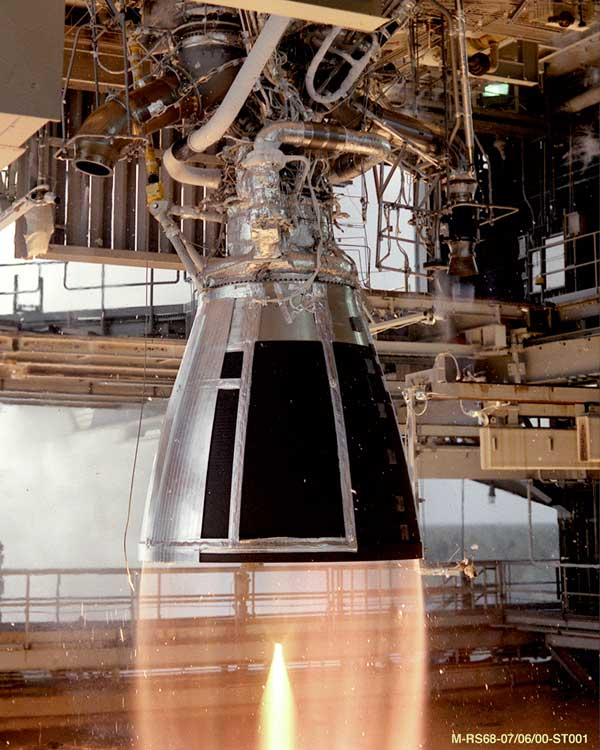
\includegraphics[height=\paperheight]{RS-68_rocket_engine_test.jpg}};
\fill[white,opacity=.91] (0,0) rectangle (595.276,89.5);
\fill[studiumInk,opacity=.96] (0,585.5) rectangle (595.276,841.89);
\node[anchor=west,text=studiumInk,font=\sffamily\bfseries\fontsize{18}{20}\selectfont,inner sep=0pt] at (51.223,38.5){STUDIUM};
\fill[studiumCyan] (51.223,61.5) rectangle (80.8,63.7);
\node[anchor=west,text=studiumInk,font=\sffamily\fontsize{9}{11}\selectfont,inner sep=0pt] at (89.49,65.5){BIBLIOTECA DE INGENIERÍA};
\node[anchor=west,text=studiumCyan,font=\sffamily\bfseries\fontsize{10}{12}\selectfont,inner sep=0pt] at (51.223,608){MANUAL UNIVERSITARIO};
\node[anchor=north west,text=white,text width=493pt,font=\rmfamily\bfseries\fontsize{33}{36}\selectfont,inner sep=0pt] at (51.223,636){#1};
\node[anchor=west,text=white!82!studiumInk,font=\sffamily\fontsize{11}{14}\selectfont,inner sep=0pt] at (51.223,732){#2};
\node[anchor=west,text=white,font=\sffamily\bfseries\fontsize{10}{12}\selectfont,inner sep=0pt] at (51.223,758){GRADO EN INGENIERÍA AEROESPACIAL};
\node[anchor=west,text=white!82!studiumInk,font=\sffamily\fontsize{10}{12}\selectfont,inner sep=0pt] at (51.223,773){Universidad de León};
\draw[white!75!studiumInk,line width=.4pt] (51.223,786) -- (544.05,786);
\node[anchor=west,text=white!82!studiumInk,font=\sffamily\fontsize{10}{12}\selectfont,inner sep=0pt] at (51.223,810){2026};
\node[anchor=east,text=white,font=\sffamily\bfseries\fontsize{10}{12}\selectfont,inner sep=0pt] at (544.05,810){I Edición};
\end{scope}\end{tikzpicture}\null\end{titlepage}\hypersetup{pageanchor=true}}

\hypersetup{pdftitle={SIMULACROS DE MOTORES COHETE},pdfauthor={Daniel Miguel Tejedor}}
\renewcommand{\studiumvolumetype}{simulacros}
\begin{document}
\studiumcover{MOTORES COHETE}{Entrenamiento y criterios de resolución}{SIMULACROS}
\frontmatter
\studiumreadingguide
\chapter*{Presentación y alcance}
\addcontentsline{toc}{chapter}{Presentación y alcance}
Este volumen pertenece al proyecto independiente de Motores Cohete, Universidad de León, curso 2026/2027. Es una elaboración original de apoyo al estudio, sin atribución de autoría ni aval a la Universidad. Los controles ejecutados y su alcance se detallan en los informes, junto con las comprobaciones pendientes.

La estructura académica conserva los seis bloques de la guía oficial. Los 28 capítulos, los problemas y los simulacros son decisiones editoriales. Los documentos proporcionados se abrieron y contrastaron; los manuscritos estudiantiles se usan para analizar competencias y posibles errores, sin copiar páginas, figuras ni enunciados extensos.

Los modelos se acompañan de hipótesis y límites. La reproducción aritmética, el álgebra simbólica, las dimensiones, la conservación y la validación experimental son niveles diferentes. Una solución de equilibrio o una curva ideal no se presenta como un ensayo real.

La procedencia técnica y los controles ejecutados se conservan en el repositorio del libro.

Se adopta $g_0=9.80665\,\mathrm{m/s^2}$ y unidades SI. Los decimales adicionales de algunas soluciones facilitan comprobar cálculos; no representan precisión experimental. Los niveles básico, intermedio, avanzado y de examen son orientativos.

Estos simulacros son originales y no son exámenes oficiales de la Universidad de León. Cada prueba propone 150 minutos y 10 puntos: cinco problemas de 2 puntos. La selección de familias y su peso son editoriales, sin atribuirlos al formato oficial.
\tableofcontents
\mainmatter
\part{Enunciados y criterios de evaluación}
\chapter{Simulacro 1}
\textbf{Tiempo orientativo: 150 minutos. Puntuación orientativa: 10 puntos.} Utilice $g_0=9.80665\,\mathrm{m/s^2}$, unidades SI y la hoja de fórmulas del manual. Identifique los supuestos, muestre despejes y compruebe al menos un balance por problema. Si detecta una limitación, explique su alcance sin inventar datos.
\section{S1.1. Tobera de Laval: geometría, régimen y prestaciones · 2 puntos}
Un modelo de gas tiene $\gamma=1.32$, $R=350$ J/(kg K), $T_c=2680$ K y $p_c=2.52$ MPa, magnitudes totales. La garganta tiene $3.220000\times10^{-4}\,\mathrm{m^2}$ y $A_e/A_t=4.44$. Para ambiente de 25 kPa, obtenga Mach, estado de salida, caudal, $c^*$, $C_F$, empuje e $I_{sp}$. Compruebe los umbrales ideales y calcule la prestación en vacío.

\section{S1.2. Superficie y garganta variables: modelo normalizado · 2 puntos}
En un modelo académico de regresión se conserva densidad, temperatura y $c^*$. La ley es $r_b/r_{ref}=(p_c/p_{ref})^n$, con $n=0.394$. Entre dos estados el área activa se multiplica por $1.49$ y la garganta por 1.02. Calcule razones de presión, regresión y caudal. Determine la razón de empuje si $C_F$ se mantiene.

\section{S1.3. Dos corrientes, duración y volumen almacenado · 2 puntos}
Un sistema académico de dos líquidos consume $7.8\,\mathrm{kg/s}$ durante $118\,\mathrm{s}$, con relación másica oxidante/combustible $3.16$. A sus estados de referencia, las densidades son 1100 y 850 kg/m$^3$. Determine caudales separados, masas consumidas, volúmenes y densidad equivalente.

\section{S1.4. Potencia, empuje y duración de maniobra · 2 puntos}
Un propulsor eléctrico académico recibe $2760\,\mathrm{W}$ con rendimiento cinético 0.60 y escape axial uniforme a $21900\,\mathrm{m/s}$. Funciona $39900\,\mathrm{s}$ sobre un vehículo de masa inicial 450 kg, sin fuerzas externas. Halle empuje, caudal, $I_{sp}$, consumo, impulso y delta-v ideal. Compare el empuje al duplicar rapidez con igual potencia.

\section{S1.5. Dos etapas: separación sin impulso · 2 puntos}
Un vehículo ideal lleva carga de 65 kg. La primera etapa tiene masa seca $140\,\mathrm{kg}$ y propulsante $720\,\mathrm{kg}$, con $c_1=2450$ m/s. La segunda tiene 40 kg secos y $200\,\mathrm{kg}$ de propulsante, con $c_2=2900$ m/s. Calcule masas de inicio y fin de cada combustión y delta-v total. Cuantifique el error de retirar la masa seca de primera etapa antes de terminar su combustión.

\section{Rúbrica orientativa} En cada problema: 0.4 puntos por frontera, hipótesis y selección de modelo; 0.6 por ecuaciones y despejes; 0.6 por sustituciones, unidades y resultados; 0.4 por comprobación e interpretación. Un error aritmético arrastrado no se penaliza de nuevo si los pasos posteriores son coherentes. Un régimen incompatible requiere revisar el modelo, aunque su aritmética cierre. Esta rúbrica es una propuesta de autoevaluación.
\chapter{Simulacro 2}
\textbf{Tiempo orientativo: 150 minutos. Puntuación orientativa: 10 puntos.} Utilice $g_0=9.80665\,\mathrm{m/s^2}$, unidades SI y la hoja de fórmulas del manual. Identifique los supuestos, muestre despejes y compruebe al menos un balance por problema. Si detecta una limitación, explique su alcance sin inventar datos.
\section{S2.1. Tobera de Laval: geometría, régimen y prestaciones · 2 puntos}
Un modelo de gas tiene $\gamma=1.32$, $R=350$ J/(kg K), $T_c=2705$ K y $p_c=2.62$ MPa, magnitudes totales. La garganta tiene $3.320000\times10^{-4}\,\mathrm{m^2}$ y $A_e/A_t=4.64$. Para ambiente de 25 kPa, obtenga Mach, estado de salida, caudal, $c^*$, $C_F$, empuje e $I_{sp}$. Compruebe los umbrales ideales y calcule la prestación en vacío.

\section{S2.2. Motor sólido: impulso, masa final y relación empuje-peso · 2 puntos}
Un motor sólido quema $260\,\mathrm{kg}$ de propulsante en $38\,\mathrm s$ con $I_{sp}=262\,\mathrm s$. La masa inerte del motor y la carga útil suman $175\,\mathrm{kg}$. Calcule el gasto medio, el empuje medio, el impulso total, la velocidad ideal y la relación empuje-peso en el encendido con la masa inicial.

\section{S2.3. Dos corrientes, duración y volumen almacenado · 2 puntos}
Un sistema académico de dos líquidos consume $8.3\,\mathrm{kg/s}$ durante $123\,\mathrm{s}$, con relación másica oxidante/combustible $3.26$. A sus estados de referencia, las densidades son 1100 y 850 kg/m$^3$. Determine caudales separados, masas consumidas, volúmenes y densidad equivalente.

\section{S2.4. Maniobra con propulsor Hall: propulsante y tiempo · 2 puntos}
Un satélite de $900\,\mathrm{kg}$ necesita $\Delta v=450\,\mathrm{m/s}$ con un propulsor Hall de $1350\,\mathrm W$, rendimiento $0.55$ e $I_{sp}=1800\,\mathrm s$. Calcule la velocidad de escape, el propulsante necesario, el empuje, el gasto y el tiempo de maniobra con empuje constante.

\section{S2.5. Dos etapas: separación sin impulso · 2 puntos}
Un vehículo ideal lleva carga de 65 kg. La primera etapa tiene masa seca $145\,\mathrm{kg}$ y propulsante $745\,\mathrm{kg}$, con $c_1=2450$ m/s. La segunda tiene 40 kg secos y $205\,\mathrm{kg}$ de propulsante, con $c_2=2900$ m/s. Calcule masas de inicio y fin de cada combustión y delta-v total. Cuantifique el error de retirar la masa seca de primera etapa antes de terminar su combustión.

\section{Rúbrica orientativa} En cada problema: 0.4 puntos por frontera, hipótesis y selección de modelo; 0.6 por ecuaciones y despejes; 0.6 por sustituciones, unidades y resultados; 0.4 por comprobación e interpretación. Un error aritmético arrastrado no se penaliza de nuevo si los pasos posteriores son coherentes. Un régimen incompatible requiere revisar el modelo, aunque su aritmética cierre. Esta rúbrica es una propuesta de autoevaluación.
\chapter{Simulacro 3}
\textbf{Tiempo orientativo: 150 minutos. Puntuación orientativa: 10 puntos.} Utilice $g_0=9.80665\,\mathrm{m/s^2}$, unidades SI y la hoja de fórmulas del manual. Identifique los supuestos, muestre despejes y compruebe al menos un balance por problema. Si detecta una limitación, explique su alcance sin inventar datos.
\section{S3.1. Tobera de Laval: geometría, régimen y prestaciones · 2 puntos}
Un modelo de gas tiene $\gamma=1.32$, $R=350$ J/(kg K), $T_c=2730$ K y $p_c=2.72$ MPa, magnitudes totales. La garganta tiene $3.420000\times10^{-4}\,\mathrm{m^2}$ y $A_e/A_t=4.84$. Para ambiente de 25 kPa, obtenga Mach, estado de salida, caudal, $c^*$, $C_F$, empuje e $I_{sp}$. Compruebe los umbrales ideales y calcule la prestación en vacío.

\section{S3.2. Presión máxima admisible y radio de perforación límite · 2 puntos}
La carcasa de un motor sólido admite una presión máxima de funcionamiento de $8.5\,\mathrm{MPa}$. El grano tiene perforación cilíndrica de $1.2\,\mathrm m$ de longitud, $\rho_p=1760\,\mathrm{kg/m^3}$, $r_{ref}=7.0\,\mathrm{mm/s}$ a $6\,\mathrm{MPa}$, $n=0.33$, $c^*=1480\,\mathrm{m/s}$ y garganta de $0.0014\,\mathrm{m^2}$. Calcule el cociente de áreas máximo y el radio de perforación máximo admisible, y la presión si la perforación llega a $0.10\,\mathrm m$.

\section{S3.3. Dos corrientes, duración y volumen almacenado · 2 puntos}
Un sistema académico de dos líquidos consume $8.8\,\mathrm{kg/s}$ durante $128\,\mathrm{s}$, con relación másica oxidante/combustible $3.36$. A sus estados de referencia, las densidades son 1100 y 850 kg/m$^3$. Determine caudales separados, masas consumidas, volúmenes y densidad equivalente.

\section{S3.4. Varios propulsores iónicos: empuje, potencia y paneles · 2 puntos}
Un remolcador necesita $0.30\,\mathrm N$ de empuje con propulsores iónicos idénticos que, cada uno, consumen $2.5\,\mathrm{kW}$ con rendimiento $0.65$ y escape de $30000\,\mathrm{m/s}$. Calcule el empuje de un propulsor, cuántos hacen falta, la potencia total, el gasto total y el área de panel si la potencia específica es $150\,\mathrm{W/m^2}$.

\section{S3.5. Dos etapas: separación sin impulso · 2 puntos}
Un vehículo ideal lleva carga de 65 kg. La primera etapa tiene masa seca $150\,\mathrm{kg}$ y propulsante $770\,\mathrm{kg}$, con $c_1=2450$ m/s. La segunda tiene 40 kg secos y $210\,\mathrm{kg}$ de propulsante, con $c_2=2900$ m/s. Calcule masas de inicio y fin de cada combustión y delta-v total. Cuantifique el error de retirar la masa seca de primera etapa antes de terminar su combustión.

\section{Rúbrica orientativa} En cada problema: 0.4 puntos por frontera, hipótesis y selección de modelo; 0.6 por ecuaciones y despejes; 0.6 por sustituciones, unidades y resultados; 0.4 por comprobación e interpretación. Un error aritmético arrastrado no se penaliza de nuevo si los pasos posteriores son coherentes. Un régimen incompatible requiere revisar el modelo, aunque su aritmética cierre. Esta rúbrica es una propuesta de autoevaluación.
\part{Soluciones completas}
\chapter{Soluciones del simulacro 1}
\section{S1.1. Tobera de Laval: geometría, régimen y prestaciones}
\begin{studiumworked}{S1.1. Tobera de Laval: geometría, régimen y prestaciones · De examen}
\textbf{Enunciado.} Un modelo de gas tiene $\gamma=1.32$, $R=350$ J/(kg K), $T_c=2680$ K y $p_c=2.52$ MPa, magnitudes totales. La garganta tiene $3.220000\times10^{-4}\,\mathrm{m^2}$ y $A_e/A_t=4.44$. Para ambiente de 25 kPa, obtenga Mach, estado de salida, caudal, $c^*$, $C_F$, empuje e $I_{sp}$. Compruebe los umbrales ideales y calcule la prestación en vacío.

\textbf{Datos.} Exponente: $1.32$; Constante específica: $350\,\mathrm{J\,kg^{-1}\,K^{-1}}$; Temperatura total: $2680\,\mathrm{K}$; Presión total: $2.520000\times10^{6}\,\mathrm{Pa}$; Garganta: $3.220000\times10^{-4}\,\mathrm{m^2}$; Expansión: $4.44$; Ambiente: $25000\,\mathrm{Pa}$.

\textbf{Incógnitas.} Estado, descarga, régimen ideal y prestaciones.

\textbf{Hipótesis.} Gas caloríficamente perfecto. Garganta ahogada, salida candidata supersónica; separación viscosa fuera del modelo.

\textbf{Modelo físico.} Área-Mach, conservación de energía y momento.
\[\varepsilon=\frac1{M_e}\left[\frac2{\gamma+1}(1+\frac{\gamma-1}2M_e^2)\right]^{(\gamma+1)/[2(\gamma-1)]}\]
\[T_e=T_c/[1+(\gamma-1)M_e^2/2],\quad p_e=p_c(T_e/T_c)^{\gamma/(\gamma-1)}\]
\[\dot m=p_cA_t/c^*,\quad F=\dot m v_e+(p_e-p_a)A_e\]
\[C_F=F/(p_cA_t),\quad I_{sp}=F/(g_0\dot m)\]
\textbf{Desarrollo.}
\begin{enumerate}
\item La raíz supersónica es $M_e=2.902686$. La raíz subsónica de igual área es $0.1328608$. De ella resulta primer bloqueo a $p_b/p_c=0.9884335$; un choque normal en salida daría $0.2793971$.
\item El ambiente tiene $p_a/p_c=0.009920635$, por debajo del umbral de choque en salida. Es compatible con divergente supersónico en el modelo unidimensional. Eso no comprueba separación viscosa.
\item La relación térmica da $1141.352\,\mathrm{K}$ y la isentrópica $74507.45\,\mathrm{Pa}$. Con la temperatura estática, $v_e=2107.806$ m/s. El área de salida es $\varepsilon A_t=0.00142968$ m$^2$.
\item El caudal crítico se obtiene de $c^*=1443.692$ m/s, luego $\dot m=0.5620588$ kg/s. El término cinético es $1184.711\,\mathrm{N}$ y el de presión $70.77981\,\mathrm{N}$.
\item La suma produce $1255.491\,\mathrm{N}$; las divisiones definitorias dan $C_F=1.547238$ e $I_{sp}=227.7777$ s. Para vacío se suma $p_aA_e$ y resulta $1291.233\,\mathrm{N}$, con $I_{sp,v}=234.2622$ s.
\end{enumerate}
\textbf{Operaciones para contrastar el cálculo.}
\begin{enumerate}

\item Magnitud 1.

\[\fitmath{y_{1}=0.562058795\cdot 2107.806294+\left(74507.4482-25000\right)\cdot 0.00142968\approx 1255.491\,\mathrm{N}}\]

\item Magnitud 2.

\[\fitmath{y_{2}=\frac{2520000\cdot 0.000322}{1443.692381}\approx 0.5620588\,\mathrm{kg/s}}\]

\item Magnitud 3.

\[\fitmath{y_{3}=1.547238088\cdot 1443.692381\approx 2233.736\,\mathrm{m/s}}\]

\end{enumerate}

\textbf{Resultados.} $M_e=2.902686$; $\dot m=0.5620588$ kg/s; $F=1255.491$ N; $C_F=1.547238$; $I_{sp}=227.7777$ s.

\textbf{Interpretación.} La geometría fija una presión de salida que no se ha igualado al ambiente. La denominación subexpandida o sobreexpandida se decide comparando esas presiones; el vacío cambia empuje de presión.

\textbf{Comprobación.} Sustituir Mach debe recuperar la relación de áreas. El caudal calculado con densidad, rapidez y área de salida coincide con el de garganta; $C_Fc^*=g_0I_{sp}$. Las dos rutas de velocidad cierran energía.

\textbf{Límites.} No se predicen capa límite, cargas laterales ni química. La compatibilidad de umbrales es del modelo inviscido y no una garantía de adherencia real.
\end{studiumworked}
\section{S1.2. Superficie y garganta variables: modelo normalizado}
\begin{studiumworked}{S1.2. Superficie y garganta variables: modelo normalizado · De examen}
\textbf{Enunciado.} En un modelo académico de regresión se conserva densidad, temperatura y $c^*$. La ley es $r_b/r_{ref}=(p_c/p_{ref})^n$, con $n=0.394$. Entre dos estados el área activa se multiplica por $1.49$ y la garganta por 1.02. Calcule razones de presión, regresión y caudal. Determine la razón de empuje si $C_F$ se mantiene.

\textbf{Datos.} Exponente local: $0.394$; Razón de área activa: $1.49$; Razón de garganta: $1.02$.

\textbf{Incógnitas.} Cocientes de presión, regresión, masa y empuje.

\textbf{Hipótesis.} Cuasiestacionario; descarga ahogada. Propiedades y CF fijos; ejemplo normalizado sin asignación a propulsante real.

\textbf{Modelo físico.} Equilibrio de generación y descarga.
\[\rho_pA_br_{ref}(p_c/p_{ref})^n=p_cA_t/c^*\]
\[P^{1-n}=\frac{A_{b,2}/A_{b,1}}{A_{t,2}/A_{t,1}}\]
\[P=(\alpha/\tau)^{1/(1-n)},\quad r_{b,2}/r_{b,1}=P^n\]
\[\dot m_2/\dot m_1=P\tau,\quad F_2/F_1=P\tau\ (C_F\ fijo)\]
\textbf{Desarrollo.}
\begin{enumerate}
\item Dividir los equilibrios elimina los parámetros dimensionales comunes. Queda $P^{1-0.394}=1.49/1.02$. Se despeja elevando a $1/(1-n)$, porque $n<1$.
\item Sustituir da $P=1.868935$. La regresión aumenta por un factor $P^n=1.279405$. El caudal generado cambia por $\alpha P^n=1.906314$.
\item La descarga produce independientemente $P\tau=1.906314$, igual al caudal generado. Con $C_F$ fijo, $F=C_Fp_cA_t$ da el mismo factor de empuje; usar sólo $P$ omitiría el cambio de garganta.
\end{enumerate}
\textbf{Operaciones para contrastar el cálculo.}
\begin{enumerate}

\item Magnitud 1.

\[\fitmath{y_{1}={\left(\frac{1.49}{1.02}\right)}^{\frac{1}{1-0.394}}\approx 1.868935\,}\]

\item Magnitud 2.

\[\fitmath{y_{2}=1.49\cdot {1.868935093}^{0.394}\approx 1.906314\,}\]

\item Magnitud 3.

\[\fitmath{y_{3}=1.868935093\cdot 1.02\approx 1.906314\,}\]

\end{enumerate}

\textbf{Resultados.} $p_2/p_1=1.868935$; $r_{b,2}/r_{b,1}=1.279405$; $\dot m_2/\dot m_1=F_2/F_1=1.906314$.

\textbf{Interpretación.} El aumento de garganta compensa parte del efecto de área activa. La hipótesis de CF fijo es adicional y podría fallar si cambia la expansión o presión ambiente.

\textbf{Comprobación.} El cierre $\alpha P^n=P\tau$ se verifica por ambas rutas. Todos los cocientes son adimensionales. Para $\alpha=\tau=1$ se recupera equilibrio inicial.

\textbf{Límites.} No se incluye almacenamiento, erosión predictiva, cinética de superficie ni inestabilidad acústica. Un exponente local no es una garantía de estabilidad real.
\end{studiumworked}
\section{S1.3. Dos corrientes, duración y volumen almacenado}
\begin{studiumworked}{S1.3. Dos corrientes, duración y volumen almacenado · De examen}
\textbf{Enunciado.} Un sistema académico de dos líquidos consume $7.8\,\mathrm{kg/s}$ durante $118\,\mathrm{s}$, con relación másica oxidante/combustible $3.16$. A sus estados de referencia, las densidades son 1100 y 850 kg/m$^3$. Determine caudales separados, masas consumidas, volúmenes y densidad equivalente.

\textbf{Datos.} Caudal total: $7.8\,\mathrm{kg/s}$; Relación de mezcla: $3.16$; Duración: $118\,\mathrm{s}$; Densidad oxidante: $1100\,\mathrm{kg/m^3}$; Densidad combustible: $850\,\mathrm{kg/m^3}$.

\textbf{Incógnitas.} Caudales, masas y volúmenes.

\textbf{Hipótesis.} Régimen constante y sólo dos corrientes. Densidades de referencia constantes; no se incluyen espacio de gas, estructura ni reservas.

\textbf{Modelo físico.} Conservación de masa y volumen de líquidos separados.
\[\dot m_f=\dot m/(1+\mathcal R),\quad \dot m_o=\mathcal R\dot m_f\]
\[m_i=\dot m_it,\quad V_i=m_i/\rho_i\]
\[\rho_{eq}=(1+\mathcal R)/(1/\rho_f+\mathcal R/\rho_o)\]
\textbf{Desarrollo.}
\begin{enumerate}
\item Se despeja combustible de $\dot m=(1+\mathcal R)\dot m_f$. Resulta $1.875\,\mathrm{kg/s}$; multiplicar por la relación da $5.925\,\mathrm{kg/s}$ de oxidante.
\item Integrar caudales constantes durante $118\,\mathrm{s}$ da $221.25\,\mathrm{kg}$ y $699.15\,\mathrm{kg}$. Dividir por densidades produce $0.2602941\,\mathrm{m^3}$ y $0.6355909\,\mathrm{m^3}$.
\item La suma de volúmenes es $0.895885\,\mathrm{m^3}$; dividir la masa total por ese volumen da $1027.364\,\mathrm{kg/m^3}$. No se ha promediado aritméticamente densidades.
\end{enumerate}
\textbf{Operaciones para contrastar el cálculo.}
\begin{enumerate}

\item Magnitud 1.

\[\fitmath{y_{1}=\frac{7.8}{1+3.16}\approx 1.875\,\mathrm{kg/s}}\]

\item Magnitud 2.

\[\fitmath{y_{2}=\left(\frac{1.875}{850}+\frac{5.925}{1100}\right)\cdot 118\approx 0.895885\,\mathrm{m^{3}}}\]

\end{enumerate}

\textbf{Resultados.} $\dot m_f=1.875$ kg/s; $\dot m_o=5.925$ kg/s; $V_p=0.895885$ m$^3$; $\rho_{eq}=1027.364$ kg/m$^3$.

\textbf{Interpretación.} La densidad equivalente es masa dividida por suma de volúmenes separados; no implica mezcla física en un depósito. La relación dada es másica y no coincide con relación volumétrica.

\textbf{Comprobación.} Los caudales suman $7.8\,\mathrm{kg/s}$ y su cociente es $3.16$. La densidad equivalente queda entre ambas densidades positivas.

\textbf{Límites.} No se predice combustión ni prestación. Si la mezcla o caudal varían, cada corriente se integra de forma independiente.
\end{studiumworked}
\section{S1.4. Potencia, empuje y duración de maniobra}
\begin{studiumworked}{S1.4. Potencia, empuje y duración de maniobra · De examen}
\textbf{Enunciado.} Un propulsor eléctrico académico recibe $2760\,\mathrm{W}$ con rendimiento cinético 0.60 y escape axial uniforme a $21900\,\mathrm{m/s}$. Funciona $39900\,\mathrm{s}$ sobre un vehículo de masa inicial 450 kg, sin fuerzas externas. Halle empuje, caudal, $I_{sp}$, consumo, impulso y delta-v ideal. Compare el empuje al duplicar rapidez con igual potencia.

\textbf{Datos.} Potencia eléctrica: $2760\,\mathrm{W}$; Rendimiento cinético: $0.6$; Rapidez uniforme: $21900\,\mathrm{m/s}$; Duración: $39900\,\mathrm{s}$; Masa inicial: $450\,\mathrm{kg}$.

\textbf{Incógnitas.} Prestaciones instantáneas e integradas.

\textbf{Hipótesis.} Haz axial monocinético, sin presión de salida. Potencia, velocidad y rendimiento constantes; masa consumida positiva menor que m0.

\textbf{Modelo físico.} Energía cinética, momento y masa variable.
\[P_j=\eta P_{el}=\dot m v_e^2/2,\quad F=\dot m v_e\]
\[F=2\eta P_{el}/v_e,\quad \dot m=2\eta P_{el}/v_e^2\]
\[m_p=\dot mt,\quad I=Ft,\quad \Delta v=v_e\ln[m_0/(m_0-m_p)]\]
\textbf{Desarrollo.}
\begin{enumerate}
\item La potencia dirigida es $1656\,\mathrm{W}$. Despejar del balance de energía da $\dot m=6.905611\times10^{-6}$ kg/s y multiplicar por velocidad produce $0.1512329\,\mathrm{N}$.
\item La conversión convencional da $I_{sp}=2233.179$ s. En el intervalo se consumen $0.2755339\,\mathrm{kg}$ y el impulso es $6034.192\,\mathrm{N s}$. La masa final es $449.7245\,\mathrm{kg}$, positiva.
\item La integración de masa variable da $13.41342\,\mathrm{m/s}$. La aproximación $I/m_0=13.40932$ m/s es algo menor porque ignora el incremento de aceleración al reducir masa.
\item Al duplicar rapidez, el empuje baja a $0.07561644\,\mathrm{N}$ y el caudal a la cuarta parte. No se ha mejorado simultáneamente tiempo de maniobra y consumo.
\end{enumerate}
\textbf{Operaciones para contrastar el cálculo.}
\begin{enumerate}

\item Magnitud 1.

\[\fitmath{y_{1}=\frac{2\cdot 0.6\cdot 2760}{21900}\approx 0.1512329\,\mathrm{N}}\]

\item Magnitud 2.

\[\fitmath{y_{2}=\frac{2\cdot 0.6\cdot 2760}{{21900}^{2}}\approx 6.905611\times10^{-6}\,\mathrm{kg/s}}\]

\item Magnitud 3.

\[\fitmath{y_{3}=21900\cdot \ln\left(\frac{450}{450-0.2755338713}\right)\approx 13.41342\,\mathrm{m/s}}\]

\end{enumerate}

\textbf{Resultados.} $F=0.1512329$ N; $\dot m=6.905611\times10^{-6}$ kg/s; $m_p=0.2755339$ kg; $\Delta v=13.41342$ m/s.

\textbf{Interpretación.} El impulso específico alto reduce consumo dentro del modelo, pero la potencia limita fuerza. La masa del sistema eléctrico sigue incluida en la masa inicial del vehículo.

\textbf{Comprobación.} $Fv_e/2=\eta P_{el}=1656$ W y $I=m_pv_e=6034.192$ N s. Para consumo pequeño, la solución logarítmica tiende a $I/m_0$.

\textbf{Límites.} No incluye gravedad, variación de potencia, divergencia, masa variable de otros consumibles ni trayectoria orbital real.
\end{studiumworked}
\section{S1.5. Dos etapas: separación sin impulso}
\begin{studiumworked}{S1.5. Dos etapas: separación sin impulso · De examen}
\textbf{Enunciado.} Un vehículo ideal lleva carga de 65 kg. La primera etapa tiene masa seca $140\,\mathrm{kg}$ y propulsante $720\,\mathrm{kg}$, con $c_1=2450$ m/s. La segunda tiene 40 kg secos y $200\,\mathrm{kg}$ de propulsante, con $c_2=2900$ m/s. Calcule masas de inicio y fin de cada combustión y delta-v total. Cuantifique el error de retirar la masa seca de primera etapa antes de terminar su combustión.

\textbf{Datos.} Seca primera: $140\,\mathrm{kg}$; Propulsante primera: $720\,\mathrm{kg}$; Seca segunda: $40\,\mathrm{kg}$; Propulsante segunda: $200\,\mathrm{kg}$; Carga: $65\,\mathrm{kg}$.

\textbf{Incógnitas.} Masas anidadas y delta-v por etapa.

\textbf{Hipótesis.} Etapas en serie, sin pérdidas ni reservas. Separación sin velocidad relativa; velocidades efectivas constantes.

\textbf{Modelo físico.} Tsiolkovski por intervalos y contabilidad de masas.
\[m_{01}=s_1+p_1+s_2+p_2+m_L,\quad m_{f1}=s_1+s_2+p_2+m_L\]
\[m_{02}=s_2+p_2+m_L,\quad m_{f2}=s_2+m_L\]
\[\Delta v=c_1\ln(m_{01}/m_{f1})+c_2\ln(m_{02}/m_{f2})\]
\textbf{Desarrollo.}
\begin{enumerate}
\item Antes de la primera combustión hay $1165\,\mathrm{kg}$. Al agotarla quedan $445\,\mathrm{kg}$, incluidos $140\,\mathrm{kg}$ secos de esa etapa. Separarla deja $305\,\mathrm{kg}$, que es la masa inicial de segunda.
\item Al terminar la segunda quedan $105\,\mathrm{kg}$. Los logaritmos son $2450\ln(1165/445)=2357.885$ m/s y $2900\ln(305/105)=3092.419$ m/s.
\item Sumar da $5450.304\,\mathrm{m/s}$. Usar $305\,\mathrm{kg}$ en el denominador del primer logaritmo daría $6375.822\,\mathrm{m/s}$, un exceso de $925.5181\,\mathrm{m/s}$. Ese exceso atribuye a la separación un efecto propulsivo que el modelo no contiene.
\end{enumerate}
\textbf{Operaciones para contrastar el cálculo.}
\begin{enumerate}

\item Magnitud 1.

\[\fitmath{y_{1}=2450\cdot \ln\left(\frac{1165}{445}\right)\approx 2357.885\,\mathrm{m/s}}\]

\item Magnitud 2.

\[\fitmath{y_{2}=2900\cdot \ln\left(\frac{305}{105}\right)\approx 3092.419\,\mathrm{m/s}}\]

\item Magnitud 3.

\[\fitmath{y_{3}=2357.885105+3092.419137\approx 5450.304\,\mathrm{m/s}}\]

\end{enumerate}

\textbf{Resultados.} $\Delta v_1=2357.885$ m/s; $\Delta v_2=3092.419$ m/s; total $5450.304$ m/s.

\textbf{Interpretación.} La segunda etapa acelera una masa inferior gracias al desprendimiento previo. La velocidad no salta al separar masa seca sin impulso.

\textbf{Comprobación.} Las diferencias de masa de cada combustión son exactamente sus propulsantes. La diferencia entre fin de primera y comienzo de segunda es exactamente $140\,\mathrm{kg}$.

\textbf{Límites.} No representa consumo paralelo, trayectoria, masa de interetapas no incluida ni variación de prestaciones con ambiente.
\end{studiumworked}
\chapter{Soluciones del simulacro 2}
\section{S2.1. Tobera de Laval: geometría, régimen y prestaciones}
\begin{studiumworked}{S2.1. Tobera de Laval: geometría, régimen y prestaciones · De examen}
\textbf{Enunciado.} Un modelo de gas tiene $\gamma=1.32$, $R=350$ J/(kg K), $T_c=2705$ K y $p_c=2.62$ MPa, magnitudes totales. La garganta tiene $3.320000\times10^{-4}\,\mathrm{m^2}$ y $A_e/A_t=4.64$. Para ambiente de 25 kPa, obtenga Mach, estado de salida, caudal, $c^*$, $C_F$, empuje e $I_{sp}$. Compruebe los umbrales ideales y calcule la prestación en vacío.

\textbf{Datos.} Exponente: $1.32$; Constante específica: $350\,\mathrm{J\,kg^{-1}\,K^{-1}}$; Temperatura total: $2705\,\mathrm{K}$; Presión total: $2.620000\times10^{6}\,\mathrm{Pa}$; Garganta: $3.320000\times10^{-4}\,\mathrm{m^2}$; Expansión: $4.64$; Ambiente: $25000\,\mathrm{Pa}$.

\textbf{Incógnitas.} Estado, descarga, régimen ideal y prestaciones.

\textbf{Hipótesis.} Gas caloríficamente perfecto. Garganta ahogada, salida candidata supersónica; separación viscosa fuera del modelo.

\textbf{Modelo físico.} Área-Mach, conservación de energía y momento.
\[\varepsilon=\frac1{M_e}\left[\frac2{\gamma+1}(1+\frac{\gamma-1}2M_e^2)\right]^{(\gamma+1)/[2(\gamma-1)]}\]
\[T_e=T_c/[1+(\gamma-1)M_e^2/2],\quad p_e=p_c(T_e/T_c)^{\gamma/(\gamma-1)}\]
\[\dot m=p_cA_t/c^*,\quad F=\dot m v_e+(p_e-p_a)A_e\]
\[C_F=F/(p_cA_t),\quad I_{sp}=F/(g_0\dot m)\]
\textbf{Desarrollo.}
\begin{enumerate}
\item La raíz supersónica es $M_e=2.943095$. La raíz subsónica de igual área es $0.1270225$. De ella resulta primer bloqueo a $p_b/p_c=0.9894212$; un choque normal en salida daría $0.2690274$.
\item El ambiente tiene $p_a/p_c=0.009541985$, por debajo del umbral de choque en salida. Es compatible con divergente supersónico en el modelo unidimensional. Eso no comprueba separación viscosa.
\item La relación térmica da $1133.749\,\mathrm{K}$ y la isentrópica $72525.98\,\mathrm{Pa}$. Con la temperatura estática, $v_e=2130.02$ m/s. El área de salida es $\varepsilon A_t=0.00154048$ m$^2$.
\item El caudal crítico se obtiene de $c^*=1450.41$ m/s, luego $\dot m=0.5997199$ kg/s. El término cinético es $1277.416\,\mathrm{N}$ y el de presión $73.21282\,\mathrm{N}$.
\item La suma produce $1350.629\,\mathrm{N}$; las divisiones definitorias dan $C_F=1.552732$ e $I_{sp}=229.6502$ s. Para vacío se suma $p_aA_e$ y resulta $1389.141\,\mathrm{N}$, con $I_{sp,v}=236.1984$ s.
\end{enumerate}
\textbf{Operaciones para contrastar el cálculo.}
\begin{enumerate}

\item Magnitud 1.

\[\fitmath{y_{1}=0.5997199178\cdot 2130.020483+\left(72525.97752-25000\right)\cdot 0.00154048\approx 1350.629\,\mathrm{N}}\]

\item Magnitud 2.

\[\fitmath{y_{2}=\frac{2620000\cdot 0.000332}{1450.41039}\approx 0.5997199\,\mathrm{kg/s}}\]

\item Magnitud 3.

\[\fitmath{y_{3}=1.552732142\cdot 1450.41039\approx 2252.099\,\mathrm{m/s}}\]

\end{enumerate}

\textbf{Resultados.} $M_e=2.943095$; $\dot m=0.5997199$ kg/s; $F=1350.629$ N; $C_F=1.552732$; $I_{sp}=229.6502$ s.

\textbf{Interpretación.} La geometría fija una presión de salida que no se ha igualado al ambiente. La denominación subexpandida o sobreexpandida se decide comparando esas presiones; el vacío cambia empuje de presión.

\textbf{Comprobación.} Sustituir Mach debe recuperar la relación de áreas. El caudal calculado con densidad, rapidez y área de salida coincide con el de garganta; $C_Fc^*=g_0I_{sp}$. Las dos rutas de velocidad cierran energía.

\textbf{Límites.} No se predicen capa límite, cargas laterales ni química. La compatibilidad de umbrales es del modelo inviscido y no una garantía de adherencia real.
\end{studiumworked}
\section{S2.2. Motor sólido: impulso, masa final y relación empuje-peso}
\begin{studiumworked}{S2.2. Motor sólido: impulso, masa final y relación empuje-peso · De examen}
\textbf{Enunciado.} Un motor sólido quema $260\,\mathrm{kg}$ de propulsante en $38\,\mathrm s$ con $I_{sp}=262\,\mathrm s$. La masa inerte del motor y la carga útil suman $175\,\mathrm{kg}$. Calcule el gasto medio, el empuje medio, el impulso total, la velocidad ideal y la relación empuje-peso en el encendido con la masa inicial.

\textbf{Datos.} $m_p=260\,\mathrm{kg}$; $t_b=38\,\mathrm s$; $I_{sp}=262\,\mathrm s$; masa inerte y carga útil $175\,\mathrm{kg}$.

\textbf{Incógnitas.} Gasto, empuje, impulso, $\Delta v$ y $F/W$.

\textbf{Hipótesis.} Gasto y empuje constantes; $I_{sp}$ constante; sin gravedad ni resistencia en el $\Delta v$.

\textbf{Modelo físico.} Ecuación del cohete y empuje medio.
\[\dot m=m_p/t_b,\quad F=I_{sp}g_0\dot m,\quad I=Ft_b\]
\[\Delta v=I_{sp}g_0\ln\frac{m_p+m_i}{m_i},\quad F/W=F/[(m_p+m_i)g_0]\]
\textbf{Desarrollo.}
\begin{enumerate}
\item El gasto es $6.84211\,\mathrm{kg/s}$ y el empuje $17579.7\,\mathrm N$; el impulso es $668029\,\mathrm{N\,s}$.
\item La velocidad ideal es $2339.54\,\mathrm{m/s}$ y la relación empuje-peso inicial $4.12099$.
\end{enumerate}
\textbf{Operaciones para contrastar el cálculo.}
\begin{enumerate}

\item Magnitud 1.

\[\fitmath{y_{1}={\left(\frac{1.54}{1.02}\right)}^{\frac{1}{1-0.404}}\approx 1.996192\,}\]

\item Magnitud 2.

\[\fitmath{y_{2}=1.54\cdot {1.996191783}^{0.404}\approx 2.036116\,}\]

\item Magnitud 3.

\[\fitmath{y_{3}=1.996191783\cdot 1.02\approx 2.036116\,}\]

\end{enumerate}

\textbf{Resultados.} $\dot m=6.84211\,\mathrm{kg/s}$; $F=17579.7\,\mathrm N$; $I=668029\,\mathrm{N\,s}$; $\Delta v=2339.54\,\mathrm{m/s}$; $F/W=4.12099$.

\textbf{Interpretación.} Una relación empuje-peso mayor que 1 permite despegar en vertical; el valor medio oculta que el empuje real varía con la forma del grano y el peso baja mientras se quema.

\textbf{Comprobación.} $I/(m_pg_0)$ devuelve $I_{sp}=262\,\mathrm s$. Con $m_p\to0$ la velocidad ideal tiende a 0.

\textbf{Límites.} No se modelan la forma de la curva empuje-tiempo, la gravedad ni la resistencia, que reducen la velocidad real.
\end{studiumworked}
\section{S2.3. Dos corrientes, duración y volumen almacenado}
\begin{studiumworked}{S2.3. Dos corrientes, duración y volumen almacenado · De examen}
\textbf{Enunciado.} Un sistema académico de dos líquidos consume $8.3\,\mathrm{kg/s}$ durante $123\,\mathrm{s}$, con relación másica oxidante/combustible $3.26$. A sus estados de referencia, las densidades son 1100 y 850 kg/m$^3$. Determine caudales separados, masas consumidas, volúmenes y densidad equivalente.

\textbf{Datos.} Caudal total: $8.3\,\mathrm{kg/s}$; Relación de mezcla: $3.26$; Duración: $123\,\mathrm{s}$; Densidad oxidante: $1100\,\mathrm{kg/m^3}$; Densidad combustible: $850\,\mathrm{kg/m^3}$.

\textbf{Incógnitas.} Caudales, masas y volúmenes.

\textbf{Hipótesis.} Régimen constante y sólo dos corrientes. Densidades de referencia constantes; no se incluyen espacio de gas, estructura ni reservas.

\textbf{Modelo físico.} Conservación de masa y volumen de líquidos separados.
\[\dot m_f=\dot m/(1+\mathcal R),\quad \dot m_o=\mathcal R\dot m_f\]
\[m_i=\dot m_it,\quad V_i=m_i/\rho_i\]
\[\rho_{eq}=(1+\mathcal R)/(1/\rho_f+\mathcal R/\rho_o)\]
\textbf{Desarrollo.}
\begin{enumerate}
\item Se despeja combustible de $\dot m=(1+\mathcal R)\dot m_f$. Resulta $1.948357\,\mathrm{kg/s}$; multiplicar por la relación da $6.351643\,\mathrm{kg/s}$ de oxidante.
\item Integrar caudales constantes durante $123\,\mathrm{s}$ da $239.6479\,\mathrm{kg}$ y $781.2521\,\mathrm{kg}$. Dividir por densidades produce $0.2819387\,\mathrm{m^3}$ y $0.7102292\,\mathrm{m^3}$.
\item La suma de volúmenes es $0.9921679\,\mathrm{m^3}$; dividir la masa total por ese volumen da $1028.959\,\mathrm{kg/m^3}$. No se ha promediado aritméticamente densidades.
\end{enumerate}
\textbf{Operaciones para contrastar el cálculo.}
\begin{enumerate}

\item Magnitud 1.

\[\fitmath{y_{1}=\frac{8.3}{1+3.26}\approx 1.948357\,\mathrm{kg/s}}\]

\item Magnitud 2.

\[\fitmath{y_{2}=\left(\frac{1.948356808}{850}+\frac{6.351643192}{1100}\right)\cdot 123\approx 0.9921679\,\mathrm{m^{3}}}\]

\end{enumerate}

\textbf{Resultados.} $\dot m_f=1.948357$ kg/s; $\dot m_o=6.351643$ kg/s; $V_p=0.9921679$ m$^3$; $\rho_{eq}=1028.959$ kg/m$^3$.

\textbf{Interpretación.} La densidad equivalente es masa dividida por suma de volúmenes separados; no implica mezcla física en un depósito. La relación dada es másica y no coincide con relación volumétrica.

\textbf{Comprobación.} Los caudales suman $8.3\,\mathrm{kg/s}$ y su cociente es $3.26$. La densidad equivalente queda entre ambas densidades positivas.

\textbf{Límites.} No se predice combustión ni prestación. Si la mezcla o caudal varían, cada corriente se integra de forma independiente.
\end{studiumworked}
\section{S2.4. Maniobra con propulsor Hall: propulsante y tiempo}
\begin{studiumworked}{S2.4. Maniobra con propulsor Hall: propulsante y tiempo · De examen}
\textbf{Enunciado.} Un satélite de $900\,\mathrm{kg}$ necesita $\Delta v=450\,\mathrm{m/s}$ con un propulsor Hall de $1350\,\mathrm W$, rendimiento $0.55$ e $I_{sp}=1800\,\mathrm s$. Calcule la velocidad de escape, el propulsante necesario, el empuje, el gasto y el tiempo de maniobra con empuje constante.

\textbf{Datos.} $m_0=900\,\mathrm{kg}$; $\Delta v=450\,\mathrm{m/s}$; $P=1350\,\mathrm W$; $\eta=0.55$; $I_{sp}=1800\,\mathrm s$.

\textbf{Incógnitas.} $v_e$, $m_p$, $F$, $\dot m$ y tiempo.

\textbf{Hipótesis.} Potencia, rendimiento e $I_{sp}$ constantes; sin fuerzas externas; empuje en la dirección del movimiento.

\textbf{Modelo físico.} Ecuación del cohete y potencia del chorro.
\[v_e=I_{sp}g_0,\quad m_p=m_0(1-e^{-\Delta v/v_e})\]
\[F=2\eta P/v_e,\quad \dot m=F/v_e,\quad t=m_p/\dot m\]
\textbf{Desarrollo.}
\begin{enumerate}
\item La velocidad de escape es $17652\,\mathrm{m/s}$ y el propulsante $22.6536\,\mathrm{kg}$.
\item El empuje es $0.0841266\,\mathrm N$, el gasto $4.76585\times10^{-6}\,\mathrm{kg/s}$ y el tiempo $4.75333\times10^{6}\,\mathrm s$, es decir, $55.0154$ días.
\end{enumerate}
\textbf{Operaciones para contrastar el cálculo.}
\begin{enumerate}

\item Magnitud 1.

\[\fitmath{y_{1}=\frac{2\cdot 0.6\cdot 2960}{22400}\approx 0.1585714\,\mathrm{N}}\]

\item Magnitud 2.

\[\fitmath{y_{2}=\frac{2\cdot 0.6\cdot 2960}{{22400}^{2}}\approx 7.079082\times10^{-6}\,\mathrm{kg/s}}\]

\item Magnitud 3.

\[\fitmath{y_{3}=22400\cdot \ln\left(\frac{450}{450-0.285994898}\right)\approx 14.24072\,\mathrm{m/s}}\]

\end{enumerate}

\textbf{Resultados.} $v_e=17652\,\mathrm{m/s}$; $m_p=22.6536\,\mathrm{kg}$; $F=0.0841266\,\mathrm N$; $t=4.75333\times10^{6}\,\mathrm s$ ($55.0154$ días).

\textbf{Interpretación.} La maniobra consume pocos kilogramos de propulsante pero dura semanas; la solución solo es válida si el satélite puede mantener la potencia disponible durante ese tiempo.

\textbf{Comprobación.} $F\,t$ dividido entre $m_0$ da una velocidad algo menor que $450\,\mathrm{m/s}$ porque ignora la pérdida de masa.

\textbf{Límites.} No se consideran eclipses, la orientación de los paneles ni el empuje fuera de la dirección del movimiento.
\end{studiumworked}
\section{S2.5. Dos etapas: separación sin impulso}
\begin{studiumworked}{S2.5. Dos etapas: separación sin impulso · De examen}
\textbf{Enunciado.} Un vehículo ideal lleva carga de 65 kg. La primera etapa tiene masa seca $145\,\mathrm{kg}$ y propulsante $745\,\mathrm{kg}$, con $c_1=2450$ m/s. La segunda tiene 40 kg secos y $205\,\mathrm{kg}$ de propulsante, con $c_2=2900$ m/s. Calcule masas de inicio y fin de cada combustión y delta-v total. Cuantifique el error de retirar la masa seca de primera etapa antes de terminar su combustión.

\textbf{Datos.} Seca primera: $145\,\mathrm{kg}$; Propulsante primera: $745\,\mathrm{kg}$; Seca segunda: $40\,\mathrm{kg}$; Propulsante segunda: $205\,\mathrm{kg}$; Carga: $65\,\mathrm{kg}$.

\textbf{Incógnitas.} Masas anidadas y delta-v por etapa.

\textbf{Hipótesis.} Etapas en serie, sin pérdidas ni reservas. Separación sin velocidad relativa; velocidades efectivas constantes.

\textbf{Modelo físico.} Tsiolkovski por intervalos y contabilidad de masas.
\[m_{01}=s_1+p_1+s_2+p_2+m_L,\quad m_{f1}=s_1+s_2+p_2+m_L\]
\[m_{02}=s_2+p_2+m_L,\quad m_{f2}=s_2+m_L\]
\[\Delta v=c_1\ln(m_{01}/m_{f1})+c_2\ln(m_{02}/m_{f2})\]
\textbf{Desarrollo.}
\begin{enumerate}
\item Antes de la primera combustión hay $1200\,\mathrm{kg}$. Al agotarla quedan $455\,\mathrm{kg}$, incluidos $145\,\mathrm{kg}$ secos de esa etapa. Separarla deja $310\,\mathrm{kg}$, que es la masa inicial de segunda.
\item Al terminar la segunda quedan $105\,\mathrm{kg}$. Los logaritmos son $2450\ln(1200/455)=2375.96$ m/s y $2900\ln(310/105)=3139.575$ m/s.
\item Sumar da $5515.534\,\mathrm{m/s}$. Usar $310\,\mathrm{kg}$ en el denominador del primer logaritmo daría $6455.661\,\mathrm{m/s}$, un exceso de $940.1265\,\mathrm{m/s}$. Ese exceso atribuye a la separación un efecto propulsivo que el modelo no contiene.
\end{enumerate}
\textbf{Operaciones para contrastar el cálculo.}
\begin{enumerate}

\item Magnitud 1.

\[\fitmath{y_{1}=2450\cdot \ln\left(\frac{1200}{455}\right)\approx 2375.96\,\mathrm{m/s}}\]

\item Magnitud 2.

\[\fitmath{y_{2}=2900\cdot \ln\left(\frac{310}{105}\right)\approx 3139.575\,\mathrm{m/s}}\]

\item Magnitud 3.

\[\fitmath{y_{3}=2375.959571+3139.574647\approx 5515.534\,\mathrm{m/s}}\]

\end{enumerate}

\textbf{Resultados.} $\Delta v_1=2375.96$ m/s; $\Delta v_2=3139.575$ m/s; total $5515.534$ m/s.

\textbf{Interpretación.} La segunda etapa acelera una masa inferior gracias al desprendimiento previo. La velocidad no salta al separar masa seca sin impulso.

\textbf{Comprobación.} Las diferencias de masa de cada combustión son exactamente sus propulsantes. La diferencia entre fin de primera y comienzo de segunda es exactamente $145\,\mathrm{kg}$.

\textbf{Límites.} No representa consumo paralelo, trayectoria, masa de interetapas no incluida ni variación de prestaciones con ambiente.
\end{studiumworked}
\chapter{Soluciones del simulacro 3}
\section{S3.1. Tobera de Laval: geometría, régimen y prestaciones}
\begin{studiumworked}{S3.1. Tobera de Laval: geometría, régimen y prestaciones · De examen}
\textbf{Enunciado.} Un modelo de gas tiene $\gamma=1.32$, $R=350$ J/(kg K), $T_c=2730$ K y $p_c=2.72$ MPa, magnitudes totales. La garganta tiene $3.420000\times10^{-4}\,\mathrm{m^2}$ y $A_e/A_t=4.84$. Para ambiente de 25 kPa, obtenga Mach, estado de salida, caudal, $c^*$, $C_F$, empuje e $I_{sp}$. Compruebe los umbrales ideales y calcule la prestación en vacío.

\textbf{Datos.} Exponente: $1.32$; Constante específica: $350\,\mathrm{J\,kg^{-1}\,K^{-1}}$; Temperatura total: $2730\,\mathrm{K}$; Presión total: $2.720000\times10^{6}\,\mathrm{Pa}$; Garganta: $3.420000\times10^{-4}\,\mathrm{m^2}$; Expansión: $4.84$; Ambiente: $25000\,\mathrm{Pa}$.

\textbf{Incógnitas.} Estado, descarga, régimen ideal y prestaciones.

\textbf{Hipótesis.} Gas caloríficamente perfecto. Garganta ahogada, salida candidata supersónica; separación viscosa fuera del modelo.

\textbf{Modelo físico.} Área-Mach, conservación de energía y momento.
\[\varepsilon=\frac1{M_e}\left[\frac2{\gamma+1}(1+\frac{\gamma-1}2M_e^2)\right]^{(\gamma+1)/[2(\gamma-1)]}\]
\[T_e=T_c/[1+(\gamma-1)M_e^2/2],\quad p_e=p_c(T_e/T_c)^{\gamma/(\gamma-1)}\]
\[\dot m=p_cA_t/c^*,\quad F=\dot m v_e+(p_e-p_a)A_e\]
\[C_F=F/(p_cA_t),\quad I_{sp}=F/(g_0\dot m)\]
\textbf{Desarrollo.}
\begin{enumerate}
\item La raíz supersónica es $M_e=2.981748$. La raíz subsónica de igual área es $0.1216801$. De ella resulta primer bloqueo a $p_b/p_c=0.990287$; un choque normal en salida daría $0.2594089$.
\item El ambiente tiene $p_a/p_c=0.009191176$, por debajo del umbral de choque en salida. Es compatible con divergente supersónico en el modelo unidimensional. Eso no comprueba separación viscosa.
\item La relación térmica da $1126.92\,\mathrm{K}$ y la isentrópica $70706.24\,\mathrm{Pa}$. Con la temperatura estática, $v_e=2151.486$ m/s. El área de salida es $\varepsilon A_t=0.00165528$ m$^2$.
\item El caudal crítico se obtiene de $c^*=1457.097$ m/s, luego $\dot m=0.6384199$ kg/s. El término cinético es $1373.551\,\mathrm{N}$ y el de presión $75.65662\,\mathrm{N}$.
\item La suma produce $1449.208\,\mathrm{N}$; las divisiones definitorias dan $C_F=1.557886$ e $I_{sp}=231.4748$ s. Para vacío se suma $p_aA_e$ y resulta $1490.59\,\mathrm{N}$, con $I_{sp,v}=238.0845$ s.
\end{enumerate}
\textbf{Operaciones para contrastar el cálculo.}
\begin{enumerate}

\item Magnitud 1.

\[\fitmath{y_{1}=0.6384199047\cdot 2151.48602+\left(70706.23977-25000\right)\cdot 0.00165528\approx 1449.208\,\mathrm{N}}\]

\item Magnitud 2.

\[\fitmath{y_{2}=\frac{2720000\cdot 0.000342}{1457.097426}\approx 0.6384199\,\mathrm{kg/s}}\]

\item Magnitud 3.

\[\fitmath{y_{3}=1.557886271\cdot 1457.097426\approx 2269.992\,\mathrm{m/s}}\]

\end{enumerate}

\textbf{Resultados.} $M_e=2.981748$; $\dot m=0.6384199$ kg/s; $F=1449.208$ N; $C_F=1.557886$; $I_{sp}=231.4748$ s.

\textbf{Interpretación.} La geometría fija una presión de salida que no se ha igualado al ambiente. La denominación subexpandida o sobreexpandida se decide comparando esas presiones; el vacío cambia empuje de presión.

\textbf{Comprobación.} Sustituir Mach debe recuperar la relación de áreas. El caudal calculado con densidad, rapidez y área de salida coincide con el de garganta; $C_Fc^*=g_0I_{sp}$. Las dos rutas de velocidad cierran energía.

\textbf{Límites.} No se predicen capa límite, cargas laterales ni química. La compatibilidad de umbrales es del modelo inviscido y no una garantía de adherencia real.
\end{studiumworked}
\section{S3.2. Presión máxima admisible y radio de perforación límite}
\begin{studiumworked}{S3.2. Presión máxima admisible y radio de perforación límite · De examen}
\textbf{Enunciado.} La carcasa de un motor sólido admite una presión máxima de funcionamiento de $8.5\,\mathrm{MPa}$. El grano tiene perforación cilíndrica de $1.2\,\mathrm m$ de longitud, $\rho_p=1760\,\mathrm{kg/m^3}$, $r_{ref}=7.0\,\mathrm{mm/s}$ a $6\,\mathrm{MPa}$, $n=0.33$, $c^*=1480\,\mathrm{m/s}$ y garganta de $0.0014\,\mathrm{m^2}$. Calcule el cociente de áreas máximo y el radio de perforación máximo admisible, y la presión si la perforación llega a $0.10\,\mathrm m$.

\textbf{Datos.} $p_{max}=8.5\,\mathrm{MPa}$; $L=1.2\,\mathrm m$; $\rho_p=1760\,\mathrm{kg/m^3}$; $r_{ref}=7.0\,\mathrm{mm/s}$ a $6\,\mathrm{MPa}$; $n=0.33$; $c^*=1480\,\mathrm{m/s}$; $A_t=0.0014\,\mathrm{m^2}$.

\textbf{Incógnitas.} $K_{n,max}$, $r_{p,max}$ y presión con $r_p=0.10\,\mathrm m$.

\textbf{Hipótesis.} Equilibrio cuasiestacionario; $A_b=2\pi r_pL$; $c^*$ constante; sin erosión.

\textbf{Modelo físico.} Inversión de la presión de equilibrio.
\[p_c=p_{ref}\left[\rho_pr_{ref}c^*K_n/p_{ref}\right]^{1/(1-n)}\]
\[K_{n,max}=\frac{p_{ref}}{\rho_pr_{ref}c^*}\left(\frac{p_{max}}{p_{ref}}\right)^{1-n},\quad r_{p,max}=\frac{K_{n,max}A_t}{2\pi L}\]
\textbf{Desarrollo.}
\begin{enumerate}
\item Se obtiene $K_{n,max}=415.555$ y $r_{p,max}=0.0771605\,\mathrm m$.
\item Para $r_p=0.10\,\mathrm m$, $K_n=538.559$ y la presión es $1.25166\times10^{7}\,\mathrm{Pa}$, es decir, $147.254\,\%$ del máximo.
\end{enumerate}
\textbf{Operaciones para contrastar el cálculo.}
\begin{enumerate}

\item Cociente de áreas máximo.

\[\fitmath{\mathrm{Kmax}=\frac{6000000}{1760\cdot 0.007\cdot 1480}\cdot {\left(\frac{8500000}{6000000}\right)}^{1-0.33}\approx 415.5547\,}\]

\item Radio máximo de perforación.

\[\fitmath{\mathrm{rpmax}=\frac{\mathrm{Kmax}\cdot 0.0014}{2\cdot \pi\cdot 1.2}}\]

\[\fitmath{\mathrm{rpmax}=\frac{(415.5546723)\cdot 0.0014}{2\cdot \pi\cdot 1.2}\approx 0.07716051\,\mathrm{m}}\]

\item Cociente de áreas con perforación de 0.10 m.

\[\fitmath{\mathrm{Kn}=\frac{2\cdot \pi\cdot 0.1\cdot 1.2}{0.0014}\approx 538.5587\,}\]

\item Presión con ese radio.

\[\fitmath{\mathrm{pc}=6000000\cdot {\left(\frac{1760\cdot 0.007\cdot 1480\cdot \mathrm{Kn}}{6000000}\right)}^{\frac{1}{1-0.33}}}\]

\[\fitmath{\mathrm{pc}=6000000\cdot {\left(\frac{1760\cdot 0.007\cdot 1480\cdot (538.5587406)}{6000000}\right)}^{\frac{1}{1-0.33}}\approx 1.251659\times10^{7}\,\mathrm{Pa}}\]

\item Cociente en por ciento respecto al máximo.

\[\fitmath{\mathrm{frac}=\frac{\mathrm{pc}}{8500000}\cdot 100}\]

\[\fitmath{\mathrm{frac}=\frac{(12516587.92)}{8500000}\cdot 100\approx 147.254\,}\]

\end{enumerate}

\textbf{Resultados.} $K_{n,max}=415.555$; $r_{p,max}=0.0771605\,\mathrm m$; con $r_p=0.10\,\mathrm m$, $p_c=1.25166\times10^{7}\,\mathrm{Pa}$ ($147.254\,\%$ del máximo).

\textbf{Interpretación.} Si la presión supera el máximo con un radio de $0.10\,\mathrm m$, el grano debe diseñarse con menos superficie o una garganta mayor; el resultado muestra hasta dónde puede avanzar la perforación.

\textbf{Comprobación.} Con $r_p=r_{p,max}$ la presión vuelve a $8.5\,\mathrm{MPa}$. El cociente supera el $100\,\%$ si $r_p>r_{p,max}$.

\textbf{Límites.} No se añade margen de seguridad estructural ni el aumento transitorio de presión del encendido; el máximo admisible es un dato.
\end{studiumworked}
\section{S3.3. Dos corrientes, duración y volumen almacenado}
\begin{studiumworked}{S3.3. Dos corrientes, duración y volumen almacenado · De examen}
\textbf{Enunciado.} Un sistema académico de dos líquidos consume $8.8\,\mathrm{kg/s}$ durante $128\,\mathrm{s}$, con relación másica oxidante/combustible $3.36$. A sus estados de referencia, las densidades son 1100 y 850 kg/m$^3$. Determine caudales separados, masas consumidas, volúmenes y densidad equivalente.

\textbf{Datos.} Caudal total: $8.8\,\mathrm{kg/s}$; Relación de mezcla: $3.36$; Duración: $128\,\mathrm{s}$; Densidad oxidante: $1100\,\mathrm{kg/m^3}$; Densidad combustible: $850\,\mathrm{kg/m^3}$.

\textbf{Incógnitas.} Caudales, masas y volúmenes.

\textbf{Hipótesis.} Régimen constante y sólo dos corrientes. Densidades de referencia constantes; no se incluyen espacio de gas, estructura ni reservas.

\textbf{Modelo físico.} Conservación de masa y volumen de líquidos separados.
\[\dot m_f=\dot m/(1+\mathcal R),\quad \dot m_o=\mathcal R\dot m_f\]
\[m_i=\dot m_it,\quad V_i=m_i/\rho_i\]
\[\rho_{eq}=(1+\mathcal R)/(1/\rho_f+\mathcal R/\rho_o)\]
\textbf{Desarrollo.}
\begin{enumerate}
\item Se despeja combustible de $\dot m=(1+\mathcal R)\dot m_f$. Resulta $2.018349\,\mathrm{kg/s}$; multiplicar por la relación da $6.781651\,\mathrm{kg/s}$ de oxidante.
\item Integrar caudales constantes durante $128\,\mathrm{s}$ da $258.3486\,\mathrm{kg}$ y $868.0514\,\mathrm{kg}$. Dividir por densidades produce $0.3039396\,\mathrm{m^3}$ y $0.7891376\,\mathrm{m^3}$.
\item La suma de volúmenes es $1.093077\,\mathrm{m^3}$; dividir la masa total por ese volumen da $1030.485\,\mathrm{kg/m^3}$. No se ha promediado aritméticamente densidades.
\end{enumerate}
\textbf{Operaciones para contrastar el cálculo.}
\begin{enumerate}

\item Magnitud 1.

\[\fitmath{y_{1}=\frac{8.8}{1+3.36}\approx 2.018349\,\mathrm{kg/s}}\]

\item Magnitud 2.

\[\fitmath{y_{2}=\left(\frac{2.018348624}{850}+\frac{6.781651376}{1100}\right)\cdot 128\approx 1.093077\,\mathrm{m^{3}}}\]

\end{enumerate}

\textbf{Resultados.} $\dot m_f=2.018349$ kg/s; $\dot m_o=6.781651$ kg/s; $V_p=1.093077$ m$^3$; $\rho_{eq}=1030.485$ kg/m$^3$.

\textbf{Interpretación.} La densidad equivalente es masa dividida por suma de volúmenes separados; no implica mezcla física en un depósito. La relación dada es másica y no coincide con relación volumétrica.

\textbf{Comprobación.} Los caudales suman $8.8\,\mathrm{kg/s}$ y su cociente es $3.36$. La densidad equivalente queda entre ambas densidades positivas.

\textbf{Límites.} No se predice combustión ni prestación. Si la mezcla o caudal varían, cada corriente se integra de forma independiente.
\end{studiumworked}
\section{S3.4. Varios propulsores iónicos: empuje, potencia y paneles}
\begin{studiumworked}{S3.4. Varios propulsores iónicos: empuje, potencia y paneles · De examen}
\textbf{Enunciado.} Un remolcador necesita $0.30\,\mathrm N$ de empuje con propulsores iónicos idénticos que, cada uno, consumen $2.5\,\mathrm{kW}$ con rendimiento $0.65$ y escape de $30000\,\mathrm{m/s}$. Calcule el empuje de un propulsor, cuántos hacen falta, la potencia total, el gasto total y el área de panel si la potencia específica es $150\,\mathrm{W/m^2}$.

\textbf{Datos.} $F_{req}=0.30\,\mathrm N$; $P_1=2.5\,\mathrm{kW}$; $\eta=0.65$; $v_e=30000\,\mathrm{m/s}$; $150\,\mathrm{W/m^2}$.

\textbf{Incógnitas.} $F_1$, número de propulsores, $P$ total, gasto y área.

\textbf{Hipótesis.} Propulsores idénticos con empuje aditivo; potencia y rendimiento constantes; toda la potencia va a los propulsores.

\textbf{Modelo físico.} Potencia de chorro por propulsor y suma.
\[F_1=2\eta P_1/v_e,\quad N=\lceil F_{req}/F_1\rceil\]
\[P=NP_1,\quad \dot m=NF_1/v_e,\quad A=P/p_{esp}\]
\textbf{Desarrollo.}
\begin{enumerate}
\item Un propulsor da $0.108333\,\mathrm N$ y el cociente $F_{req}/F_1=2.76923$ obliga a usar $3$ propulsores.
\item La potencia total es $7500\,\mathrm W$, el gasto $1.08333\times10^{-5}\,\mathrm{kg/s}$ y el panel tiene $50\,\mathrm{m^2}$.
\end{enumerate}
\textbf{Operaciones para contrastar el cálculo.}
\begin{enumerate}

\item Magnitud 1.

\[\fitmath{y_{1}=\frac{2\cdot 0.6\cdot 3160}{22900}\approx 0.1655895\,\mathrm{N}}\]

\item Magnitud 2.

\[\fitmath{y_{2}=\frac{2\cdot 0.6\cdot 3160}{{22900}^{2}}\approx 7.230983\times10^{-6}\,\mathrm{kg/s}}\]

\item Magnitud 3.

\[\fitmath{y_{3}=22900\cdot \ln\left(\frac{450}{450-0.2957472207}\right)\approx 15.0552\,\mathrm{m/s}}\]

\end{enumerate}

\textbf{Resultados.} $F_1=0.108333\,\mathrm N$; $N=3$; $F=0.325\,\mathrm N$; $P=7500\,\mathrm W$; $A=50\,\mathrm{m^2}$.

\textbf{Interpretación.} El número se redondea hacia arriba y el empuje real supera el requerido; con tres propulsores se necesita un panel grande, que domina la masa del sistema.

\textbf{Comprobación.} El cociente $F_{req}/F_1$ es menor que 3 y mayor que 2, de modo que 3 es el mínimo entero.

\textbf{Límites.} No se incluyen la potencia de los demás sistemas, la degradación del panel ni el funcionamiento a potencia parcial.
\end{studiumworked}
\section{S3.5. Dos etapas: separación sin impulso}
\begin{studiumworked}{S3.5. Dos etapas: separación sin impulso · De examen}
\textbf{Enunciado.} Un vehículo ideal lleva carga de 65 kg. La primera etapa tiene masa seca $150\,\mathrm{kg}$ y propulsante $770\,\mathrm{kg}$, con $c_1=2450$ m/s. La segunda tiene 40 kg secos y $210\,\mathrm{kg}$ de propulsante, con $c_2=2900$ m/s. Calcule masas de inicio y fin de cada combustión y delta-v total. Cuantifique el error de retirar la masa seca de primera etapa antes de terminar su combustión.

\textbf{Datos.} Seca primera: $150\,\mathrm{kg}$; Propulsante primera: $770\,\mathrm{kg}$; Seca segunda: $40\,\mathrm{kg}$; Propulsante segunda: $210\,\mathrm{kg}$; Carga: $65\,\mathrm{kg}$.

\textbf{Incógnitas.} Masas anidadas y delta-v por etapa.

\textbf{Hipótesis.} Etapas en serie, sin pérdidas ni reservas. Separación sin velocidad relativa; velocidades efectivas constantes.

\textbf{Modelo físico.} Tsiolkovski por intervalos y contabilidad de masas.
\[m_{01}=s_1+p_1+s_2+p_2+m_L,\quad m_{f1}=s_1+s_2+p_2+m_L\]
\[m_{02}=s_2+p_2+m_L,\quad m_{f2}=s_2+m_L\]
\[\Delta v=c_1\ln(m_{01}/m_{f1})+c_2\ln(m_{02}/m_{f2})\]
\textbf{Desarrollo.}
\begin{enumerate}
\item Antes de la primera combustión hay $1235\,\mathrm{kg}$. Al agotarla quedan $465\,\mathrm{kg}$, incluidos $150\,\mathrm{kg}$ secos de esa etapa. Separarla deja $315\,\mathrm{kg}$, que es la masa inicial de segunda.
\item Al terminar la segunda quedan $105\,\mathrm{kg}$. Los logaritmos son $2450\ln(1235/465)=2393.133$ m/s y $2900\ln(315/105)=3185.976$ m/s.
\item Sumar da $5579.108\,\mathrm{m/s}$. Usar $315\,\mathrm{kg}$ en el denominador del primer logaritmo daría $6533.297\,\mathrm{m/s}$, un exceso de $954.1887\,\mathrm{m/s}$. Ese exceso atribuye a la separación un efecto propulsivo que el modelo no contiene.
\end{enumerate}
\textbf{Operaciones para contrastar el cálculo.}
\begin{enumerate}

\item Magnitud 1.

\[\fitmath{y_{1}=2450\cdot \ln\left(\frac{1235}{465}\right)\approx 2393.133\,\mathrm{m/s}}\]

\item Magnitud 2.

\[\fitmath{y_{2}=2900\cdot \ln\left(\frac{315}{105}\right)\approx 3185.976\,\mathrm{m/s}}\]

\item Magnitud 3.

\[\fitmath{y_{3}=2393.132667+3185.975637\approx 5579.108\,\mathrm{m/s}}\]

\end{enumerate}

\textbf{Resultados.} $\Delta v_1=2393.133$ m/s; $\Delta v_2=3185.976$ m/s; total $5579.108$ m/s.

\textbf{Interpretación.} La segunda etapa acelera una masa inferior gracias al desprendimiento previo. La velocidad no salta al separar masa seca sin impulso.

\textbf{Comprobación.} Las diferencias de masa de cada combustión son exactamente sus propulsantes. La diferencia entre fin de primera y comienzo de segunda es exactamente $150\,\mathrm{kg}$.

\textbf{Límites.} No representa consumo paralelo, trayectoria, masa de interetapas no incluida ni variación de prestaciones con ambiente.
\end{studiumworked}
\section*{Alcance de la comprobación}\addcontentsline{toc}{chapter}{Alcance de la comprobación} Los resultados se recalcularon mediante SymPy y los modelos de descarga, masa y energía se sometieron a controles separados. No se utilizan soluciones manuscritas como referencia numérica. Los tiempos y puntuaciones son orientativos y no predicen requisitos futuros de la asignatura.\end{document}
